
%%% Local Variables:
%%% mode: latex
%%% TeX-master: t
%%% End:

\chapter{标签化地址空间}
\label{chap:labeladdrspace}

当前数据中心虚拟化、多租户的使用场景给服务器提出了区分化服务的需求。
实现区分化服务,首先需要使硬件识别出不同的应用,并能够获得不同应用的服务质量需求信息。
传统的服务器无法提供这样的功能,虽然服务器上运行着不同的应用,
硬件却不能对这些应用进行区分,只能进行无差别的处理,无法满足应用不同的服务质量需求。
造成这一现状的原因是当前计算机体系结构在设计之初并没有考虑多租户使用场景,
硬件部件与数据通路中没有提供基于应用的区分和隔离功能,
要解决这一问题,需要让体系结构提供一种软硬件的接口,
实现硬件层次的应用区分以及软硬件之间的需求信息传递,
消除软硬件之间的信息鸿沟。

本章提出了标签化地址空间的设计,
使用统一标签区分不同应用,并为计算机系统内所有请求标识应用标签,
通过标签机制打破目前体系结构中软硬件之间的信息鸿沟,
将应用的需求信息传递到硬件。
硬件也不再需要通过猜测的方式区分应用,
可以直接利用标签信息实现应用区分与区分化处理。
本章内容安排如下:
首先分析应用区分信息在体系结构内传播的必要性与难点,
之后讨论本文所提出的标签化地址空间的原理、实现难点、以及技术优势; 
最后在模拟器平台上实现了标签化地址空间,
并利用标签化地址空间提供的应用区分功能实现无软件干预的全硬件支持虚拟化
(类似于NoHype工作\cite{keller_nohype:_2010})。

%
% 本章结构:
%
% -> 现有系统如何共享资源
%    |-> 资源包括 cpu/mem/io
%        |->基于请求源的区分(划分,调度)
% -> 问题:丢失信息,带来性能问题
%    |-> TLB问题,切换address space时需要刷tlb
%    |-> cache / mem / bus / io 竞争
% -> TLB通过加标签解决,I/O可以调度,但cache/mem/bus没办法
% -> 原因是没有标签
% -> 增加标签化地址空间
% 
% -> 标签化地址空间实现:标记与传播
% -> 应用:NoHype
% -> Intel技术方案对比
% -> 小结:标签化地址空间是未来体系结构的基础
%

\section{问题分析}

本章主要讨论多应用共享场景下的区分化服务,
其本质是如何在共享环境下实现资源隔离,
首先讨论现有体系结构下硬件资源共享的现状。

在计算机中,处理器、内存和I/O是三类最主要的共享资源,
现有的体系结构已经实现了对这三类资源以进程或虚拟机为粒度的隔离。
其中处理器资源的隔离相对比较简单,一般采用处理器核静态分配或基于时间片的应用调度实现隔离;
相比之下,内存与I/O资源的隔离则略显复杂,下面将分别对这两类资源的共享与隔离方式进行讨论。

\textbf{内存资源共享}\quad	% 进程或虚拟机粒度,通过地址空间隔离实现资源隔离
不同的进程拥有独立的地址空间,
现代处理器通过内存管理单元(Memory Management Unit,MMU)实现不同进程地址空间的隔离。
软件代码使用虚拟地址进行访存,MMU通过分页或分段机制将虚拟地址转换为物理地址后,
发往内存控制器。
操作系统负责分配并管理MMU的地址映射,
将不同进程的虚拟地址空间映射到不同的物理地址空间,实现地址空间的隔离。
以Intel-IA架构处理器为例,操作系统(如Linux)仅使用处理器提供的分页机制实现地址映射,
内核负责维护地址映射所需的页表,并通过处理器CR3寄存器将页表地址传递给硬件MMU。
以进程为粒度进行地址空间隔离,实现内存资源的隔离。
虚拟化技术出现后,处理器中引入了扩展页表(Extended Page Table, EPT)机制,
在原有的两级分页的基础上增加一级从客户机物理地址(guest-physical address)到
主机物理地址(host-physical address)的映射,
将内存资源隔离的粒度从进程扩大到虚拟机。

\textbf{I/O资源共享}\quad	% 通过软件在访问端实现隔离
对于I/O资源,操作系统或VMM负责管理整个系统中的I/O设备。
以Linux操作系统为例,由内核实现对I/O设备的管理与操作,
并通过文件的形式为应用提供I/O设备的访问接口;
虚拟化场景下也是类似,由VMM负责管理所有的I/O设备,
通过软件模拟虚拟设备的方式实现虚拟机之间I/O设备的共享。
以上两种方式都是在共享的操作系统内核或VMM,通过调度的方式实现I/O资源的共享与隔离。

总结来说,目前系统中普遍在请求源(处理器)实现内存与 I/O资源的共享管理,
通过调度的方式将不同应用对共享资源的访问划分到不同的位置或不同的时间实现资源隔离。
虽然这种方式能够实现硬件资源的共享与隔离,但却造成了硬件层次上应用信息的丢失:
内存资源共享相当于将多个应用的地址空间映射到同一个物理地址空间,
内存控制器收到的是对该物理地址空间的访问,而无法区分出请求的来源;
I/O资源的访问经过操作系统或VMM的转换,
使得I/O设备实际收到的是来自于操作系统或VMM的请求,也丢失了应用的信息。

应用信息的丢失同样会造成正确性与性能方面的问题。
以MMU为例,它使用TLB缓存最近访问过的页表以加速地址映射,
由于TLB是按照虚拟地址进行索引的,这使得具有相同虚拟地址的不同进程在TLB中可能存在冲突。
其他一些使用虚拟地址进行索引的缓存结构也存在相类似的问题,这里仅以TLB为例进行说明。
为了防止出现正确性问题,早期的解决方案是在地址空间切换时清空所有的TLB记录,
但这种清空操作的开销过大,会对地址空间切换的性能造成影响;
为了解决这一问题,x86架构提出了PCIDs(Process-Context Identifiers),
将地址空间标识记录到TLB表项中,让TLB能够同时缓存多个地址空间的映射信息,
通过区分不同地址空间实现在地址空间切换时无需清空所有的TLB表项。
在虚拟机引入后,多个虚拟机具有相同的客户机物理地址,也产生了相同的问题,
解决方案也是类似:在TLB中增加VPID(Virtual Processor Identifier)标识,
实现不同虚拟机的区分,消除不必要的TLB清空操作,降低虚拟机切换的开销。
通过以上2个例子可以发现,无论是PCID还是VPID,
都是将应用的标识传递到共享硬件(如TLB,Cache),并通过应用区分避免不必要的操作,降低开销。

除TLB外,应用信息的丢失使得处理器末级缓存、内存控制器、
系统总线或I/O设备等位置都会出现性能问题,
不同应用对这些共享资源的竞争会带来严重的性能损失,
如第\ref{chap:background}章中给出的Intel的数据表明,
在末级缓存上的竞争最大会带来50\%的性能损失\cite{}。
可以通过软件层次的调度缓解I/O设备上的竞争,
但处理器末级缓存、内存与系统总线这类不受软件控制的硬件部件,竞争无法避免,
特别是随着处理器核心数量的不断增加,这种多应用共享竞争的情况会越来越严重。
要解决这一问题,唯一的办法就是在这些硬件部件内部对来自不同应用的请求进行区分化处理,
其前提就是将应用的信息传递到硬件。

本文使用标签作为应用信息的载体,标签伴随请求在整个计算机系统内传播,
在体系结构原有地址空间之外,额外的增加了用于应用区分的``标签化地址空间''。
标签化地址空间是PARD体系结构的基础,通过将应用标签传递到体系结构内所有的硬件部件中,
可以让这些共享的硬件部件能够识别出不同的应用,实现应用的资源隔离与性能隔离。
通过标签化地址空间以及少量的硬件修改,PARD可以很容易的将一台计算机划分为多个相互隔离的逻辑域,
在无需虚拟化软件(如KVM、Xen、VMware等)的辅助下,即可直接将这些逻辑域作为虚拟机使用;
同时,硬件能够通过标签获得更多来自上层应用的信息,辅助其调整自身的策略,以更好的服务应用。

但将标签信息并不能简单的传播到整个计算机,
其间需要涉及到不同总线协议之间的转换,并可能会带来请求的合并与拆分;
请求在经过带有缓存功能的部件(如处理器末级缓存、I/O Cache、各种队列buffer等)时,
可能会丢失标签信息;
另外,系统中除了处理器外,多应用共享的I/O设备也会向外发出请求,包括DMA与中断,
如何为这样的请求传播正确的标签也是一个困难的问题。


\section{标签机制}

在之前的章节中已经对PARD的标签机制进行了介绍,简单来说其核心包括2点:
一是如何为计算机中的请求\textbf{标记}上正确的标签,
二是保证标签在整个计算机系统中正确\textbf{传播}。
但在具体实现标签机制时,仍然有一些问题需要考虑,
本节主要讨论其中的标记问题,传播问题将在下一节中讨论。


\subsection{标签粒度与格式}

PARD对用户提供了逻辑域抽象,因此简单的标签方案可以直接将一个逻辑域映射到为一个标签,
以逻辑域为粒度分配系统内的硬件资源,并对共享硬件资源的访问进行控制,
本文所设计的FPGA原型系统(参见第\ref{chap:impl}章)选择该方案进行实现。
另一些应用,需要为逻辑域内不同应用设定不同的资源访问级别,
基于容器的技术的轻量级虚拟化即属于该类型,运行在不同容器中的应用虽然具有不同的优先级,
但它们能够访问相同的资源。
为了支持这种类型的应用,本文提出了两级标签的概念,如图\ref{fig:tagging-format}所示,
将标签划分为资源域与性能域两部分,
不同资源域的应用在硬件资源上相互隔离,且具有不同的性能策略;
具有相同资源域的应用共享同一份硬件资源,
但这些共享的硬件资源使用不同的性能策略来处理来自不同性能域的应用。

使用两级标签区分相同逻辑域内不同应用时,由于应用之间存在共享的代码,如操作系统内核、共享库和系统进程(e.g. pdflush)。
共享库虽然是同一份代码,但是它被映射到不同的进程地址空间,因此在执行时使用不同的性能域,天然的实现了区分。
从用户态进入内核态存在2种可能,一是应用通过系统调用主动陷入内核执行,二是中断或异常入口。
对于系统调用入口,因为是应用主动进入,因此无需进行性能域切换,直接使用当前性能域即可。
对于中断或异常入口,由于无法确定是由哪个应用引起,所以不能将其划分到任何一下应用的性能域,
因此为这种情形单独分配一个性能域标签;
同时为了防止引起中断或异常的是优先级较高的应用,而且内核处理时间通常不会特别长,
这个特殊的性能域标签被赋予最高优先级。


\begin{figure}[htb]
  \centering
  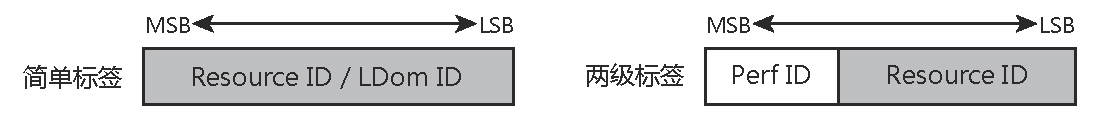
\includegraphics[width=\textwidth]{label/tagging-format}
  \caption[标签格式]{标签格式:分为简单标签与两级标签,
    简单标签直接将逻辑域(LDom ID)映射为标签,
    两级标签将标签分为资源域(Resource ID)和性能域(Perf ID)两部分。
    只有两级标签的性能域部分可以由用户进行修改,
    简单标签或两级标签的资源域(图中阴影部分)只能通过PRM进行修改,
    以保证硬件资源分配不会出现冲突。}
  \label{fig:tagging-format}
\end{figure}

\subsection{如何为请求打标签}
\label{chap:labeladdrspace:tagging}
在确定了标签的格式与内容后,需要将该标签标记到对应的请求上。
在计算机中存在两类请求源:处理器核与I/O设备的DMA引擎,
需要对他们进行分别处理。

\begin{figure}[tb]
\begin{minipage}{0.48\textwidth}
  \centering
  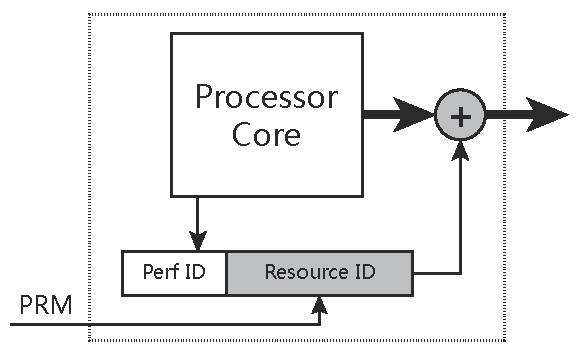
\includegraphics[width=0.9\textwidth]{label/tagging-core-request}
  \caption{为处理器核请求打标签}
  \label{fig:tagging-core-request}
\end{minipage}\hfill
\begin{minipage}{0.48\textwidth}
  \centering
  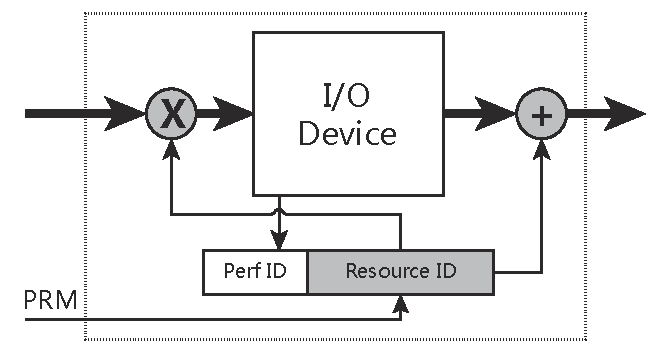
\includegraphics[width=0.9\textwidth]{label/tagging-io-request}
  \caption{为I/O请求打标签}
  \label{fig:tagging-io-request}
\end{minipage}
\end{figure}

\textbf{处理器核}\quad
为实现处理器核发出的请求的标记,
需要在处理器核内增加一个标签寄存器,将当前正在使用该处理器核的应用标签保存在该寄存器中。
对于简单标签模式,该寄存器对处理器核不可见,只能通过PRM在逻辑域切换时进行修改;
对于两级标签模式,该寄存器的性能域部分对处理器可见,
可以由逻辑域内的操作系统在应用切换时进行修改,而资源域与简单模式下相同,只能由PRM进行修改。
图\ref{fig:tagging-core-request}给出了两级标签模式下,处理器核的请求标记过程:
处理器核发出的请求与标签寄存器的值进行组成,形成带有标签的请求发送到外部;
标签寄存器的资源域部分只能由PRM进行修改,性能域部分可以通过处理器核进行修改。

\textbf{I/O与中断请求}\quad
对于I/O访问,有两种访问模式,即Programmed-I/O(PIO)和Directed Memory Access(DMA)。
对于PIO访问请求,由于I/O请求已经在处理器核端进行了标记,
因此在设备端直接将请求所附带的标签返回即可,但对于DMA请求进行标签标记则需要进行额外的处理。

在介绍PARD的DMA请求标签机制前,先对DMA的工作原理进行简要回顾。
通常一个DMA请求过程可以分为3个阶段:
首先设备驱动发送一个``DMA描述符''首地址到DMA控制器,
该``DMA描述符''包含了DMA的缓存信息,例如起始地址、缓存大小、状态;
当初始化完成之后,DMA控制器加载描述符,从中获取每个DMA操作必要的信息并开始数据传输;
最后当所有数据都传输完成后,DMA控制器产生中断告诉CPU数据处理完成。

为了实现DMA请求的标签机制,PARD在每个DMA控制器中都加入一个``标签寄存器'',
如图\ref{fig:tagging-io-request}所示。
在逻辑域创建过程中,PRM对设备进行分配,将逻辑域的资源标签写入到该标签寄存器中。

对于DMA请求的3个步骤,标签寄存器相应的操作如下:

\begin{enumerate}[leftmargin=2\parindent, nolistsep, label=\arabic*)]
  \item 初始化标签寄存器性能域并读取DMA描述符。当设备驱动向DMA引擎写如DMA描述符信息的同时,
        将请求相关的标签性能域部分写入到标签寄存器中,
        DMA引擎将标签寄存器中的值附加到DMA描述符读取请求中;
  \item 标记数据传输请求。当设备的DMA引擎与内存控制器进行收发数据时,
        从其标签寄存器中取出标签,将每个数据传输请求上都打该标签;
  \item 标记中断信号。对于中断,PARD对当前的中断控制器
        (Advanced Programmable Interrupt Controller, APIC)进行适当的扩充。
        在APIC中增加多个中断映射表,其中的每一个都与一个应用标签进行关联。
        这样当DMA引擎将要产生一个中断时,把应用标签标记到中断请求中,然后发往APIC。
        APIC使用请求中的应用标签来获取相关的映射表,
        根据表中的信息将中断请求转发给指定的处理器核。
\end{enumerate}



\section{标签传播}
\label{chap:labeladdrspace:propagation}

标签需要伴随请求在整个生命周期中传播,
这些不同类型的请求需要在各种协议类型的总线上传播(如QPI/HT、AXI、PCI-E等),
其间需要进行多次协议转换,同时会多次穿过各种Cache与Buffer,
本节首先讨论如何扩展现有的总线架构,使其能够传递标签信息,并讨论如何在保证在传播过程中请求与标签始终匹配。
%计算机中的请求主要分为三类:处理器发出的读写请求、I/O设备发出的DMA请求、中断请求。

% TODO: Rewrite this
%\subsection{总线与协议转换}
%
%不同总线上如何实现地址空间

% 总线都是基于包的

% Up-size/Down-size时要注意标签归属


\subsection{多阶段写回请求}
\label{chap:labeladdrspace:propagation:cache}

为了提高性能,计算机数据通路中采用写回(writeback)机制的写操作通常会被拆分成多个阶段。
以共享末级缓存为例,写请求的第1阶段只是将数据写入到缓存中,并将其所属的数据块标记为脏块,
只有当缓存缺失发生且该数据块被选择为替换备选时,数据才会被真正写回到内存。
如果仅使用末级缓存所接收到请求的应用标签作为写回请求的标签,可能会产生标签错误:
引起写回操作数据所属的应用与被写回的数据所属的应用不一致。
为了防止这种情况的发生,需要在共享末级缓存中,
为所有缓存的数据块额外记录其所属应用的标签Owner-DSid,
在第1阶段数据被写入缓存时,将写请求中包含的DSid记录为其Owner-DSid;
当写回操作发生时,使用其Owner-DSid作为传递到下一级的标签。
其他与共享末级缓存行为类似的具有写回机制的部件,都需要应用以上的修改,
才能保证请求在通过该部件后保证应用标签的正确性。


\subsection{一致性协议}

% 侦听和目录两种协议,目前大都使用目录(扩展性原因)
% Source-Snooping 1-2 sockets    <= need reference
% Home-Snooping   4+ sockets
% Directory       64+
PARD使用共享内存多处理器架构,每个处理器都包含自己的私有缓存,
需要使用一致性协议来保证这些私有缓存的一致性。
最常用的保持一致性的方法是基于侦听或基于目录,它们各有优缺点,
基于侦听的方法的优势是响应速度快,所有的请求通过一次广播的请求和回应即可完成,
但它带来的问题是链路带宽占用过大,尤其是当核数增加时,其带宽占用也越来越大。
基于目录的方法主要解决带宽占用问题,通过使用一个公共的目录来记录所有数据的缓存情况,
在需要执行无效操作时,只将请求发送到包含该数据的节点,可以使用点对点的连接,
而无需广播,降低的带宽占用,但与此同时也增加了响应延迟
(需要request/forward/respond三跳)。
通常在四核以下使用基于侦听的方法实现一致性协议,
而更多的核数后需要使用基于目录的方法以降低开销。

% PARD需要对目录项进行修改,以保证正确性
当前处理器核数不断增加,目前普遍的服务器都具有24个处理器核,
这些服务器大都采用基于目录的一致性。
%图\ref{}是基于目录的一致性协议的执行流程,首先....。
由于PARD使用标签的方式区分不同逻辑域的地址空间,系统中存在多个重叠的地址空间,
应用标签是区分这些重叠地址空间的唯一标识。
因此,PARD修改一目录项的定义,将标签信息也加入到目录项中,
在进行地址对比时需要同时对比地址与标签,只有两都同时匹配时才将请求转发到该结点。

% 云计算场景下,每个虚拟机核数较少,可以使用局部侦听的方法实现快速的一致性,
% 同时开销也可控
再次考察基于侦听的一致协议,在节点数较少时性能要高于目录一致性协议,
而随着服务器中核数增加,链路带宽不足以满足侦听需求,
因此才被抛弃,转而使用实现更为复杂的目录一致性协议。
当前多租户云计算场景下,虽然服务器本身具有大量的处理器核(>24),
但每个用户的虚拟机通常只使用很少数量的处理器核\cite{}。    % <= TODO: need reference
由于虚拟机之间无内存共享,因此可以只在所有处理器的一个子集中实现一致性,
在这样的范围下,使用基于侦听的一致性可以提高性能,同时由于节点数目较少,
广播开销也不大;特别的,当只使用一个处理器核时,可以忽略所有一致性相关的请求,
进一步降低一致性开销。

PARD的标签化地址空间为以上的一致性协议提供了支持,
即只需要将一致性请求发送到与其标签相同的处理器核,
而无需在全局范围内广播或进行目录查询操作,
通过缩小一致性范围,降低一致性开销并提高性能。

% 即使虚拟机的核数较多,也可以使用局部目录一致性,降低目录存储开销

% 结论,标签化地址空间以及逻辑域抽象,可以实现局部一致性协议,
% 通用逻辑域核数决定一致性协议的类型(甚至是不需要一致性,单核)

\subsection{多内存控制器}

随着处理器核数不断增长,单个内存控制器性能无法满足处理器核的需求,
现有体系结构实现通常包括多个内存控制器,
处理器需要提供一种机制实现物理地址空间在多个内存控制器的分布,
并为请求提供地址解码支持。
以Intel的Xeon架构为例,其使用Source Address Decoder(SAD)
和Target Address Decoder(TAD)实现地址空间管理\cite{intel-xeon-7500}。
其中SAD位于Cache Box(Cbox),负责将请求地址解析到对应的I/O或内存控制器
(对于interleave的地址,则是一组控制器),本节主要讨论对内存地址的解码;
而TAD位于Home Agent(Bbox),负责将请求地址解析为本地地址(主要是处理interleave情况),
并将解析后的地址发送给内存控制器(Mbox)完成访存请求。

SAD的结构如图\ref{fig:intel-7500-sad}所示,
其中包含一个20项的译码表,输入为请求地址,
输出为路由目的地列表,并交给Router模块转发请求。
在Intel的这种体系结构下,请求路由是由请求地址决定。
在PARD体系结构下,需要综合考虑请求地址与应用标签,
因此需要对译码表进行扩充,在系统中预留多组译码表(组数由支持的最大逻辑域数量决定),
这些译码表使用逻辑域标签进行索引,当PRM决定在某个处理器核上运行逻辑域时,
将该逻辑域对应的译码表加载到处理器中,
这样保证该处理器核在做地址译码时使用对应用逻辑域的地址分配。

\begin{figure}[tb]
  \centering
  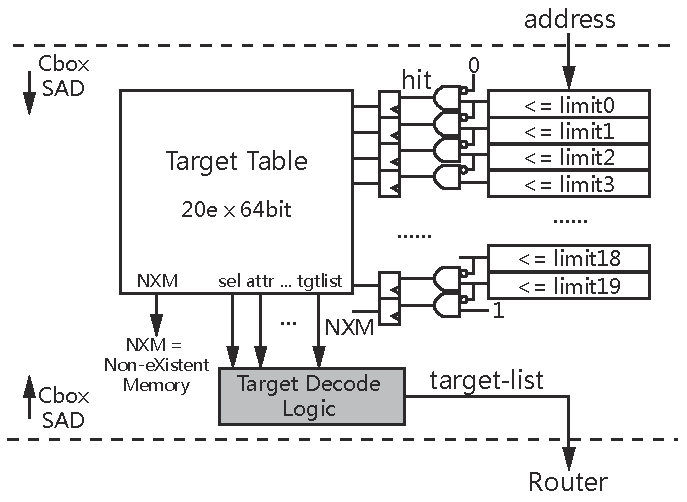
\includegraphics[width=0.7\textwidth]{label/intel-7500-sad}
  \caption[Intel SAD地址译码]{Intel SAD地址译码\cite{intel-xeon-7500}}
  \label{fig:intel-7500-sad}
\end{figure}


\section{PARD模拟器}
\label{chap:labeladdrspace:nohype}

利用本章所设计的标签化地址空间架构,通过应用标签以及相应的标签传播机制,
在整个计算机体系结构内能够识别出来自不同应用的请求。
本节基于模拟器,介绍标签机制的具体实现,
并讨论如何该架构下实现全硬件支持的虚拟化技术,提供PARD体系结构的逻辑域抽象。

PARD模拟器是基于gem5\cite{binkert_gem5_2011}开发的时钟精确(cycle-accurate)
体系结构模拟器\footnote{PARD-gem5模拟器已在LGPL协议下开源,地址https://github.com/fsg-ict/PARD-gem5},
它使用x86指令集与Classic Memory内存模型,
能够支持atomic、timing-simple和detail 3种模型进行仿真。
它模拟了1台四核x86服务器,具体配置参数如表\ref{tab:pard-sim-setup}所示,
主要包括:
处理器核使用乱序四发射,工作频率为2GHz,
具有分离的指令与数据缓存,容量均为64KB;
4个处理器核共享4MB的末级缓存(16路组相连)和1个DDR3内存控制器,内存容量为8GB;
在I/O方面,服务器提供4个IDE控制器,每个控制器上挂载2个磁盘。

\begin{table}[b]
  \centering
  \begin{minipage}[t]{0.9\linewidth}
  \caption{PARD模拟器参数}  
  \label{tab:pard-sim-setup}
    \begin{tabular*}{\linewidth}{rl}
      \toprule[1.5pt]
      CPU                  & 4 4-issue Out-of-Order X86 cores, 2GHz\\
      L1-I/core            & 64KB 2-way, hit = 2 cycles \\
      L1-D/core            & 64KB 2-way, hit = 2 cycles \\
      Shared LLC           & 4MB 16-way, hit = 20 cycles \\
      \hline
      DRAM                 & 8GB DDR3-1600 11-11-11, 4Gbit chip (Micron MT41J512M8) \\
                           & 1 channel, 2 ranks/channel, 8 banks/Rank \\
                           & Burst Length = 8, Row buffer = 1KB \\
                           & tCK=1.25ns, tRCD = 13.75ns, tCL = 13.75ns, tRP = 13.75ns, tRAS = 35ns, \\
                           & tRRD = 6ns \\
      \hline
      Disks                & 4-channel IDE controller, 8 disks \\
      \hline
      Platform             & 100MHz X86 core, 16MB DRAM, 32MB Flash Storage \\
      Resource             & 1 Ethernet adaptor  \\
      Manager              & 4 control plane adaptors (CPA) \\
      (PRM)                & Firmware: tailored Linux kernel 2.6.28.4 with Busybox \cite{busybox} \\
      \hline
      Server OS            & Gentoo Linux with kernel 2.6.28.4 \\
      \hline
      Workloads            & memcached \cite{memcached}, SPEC-CPU 2006 \cite{cpu2006} \\
                           & MicroBenchmark: CacheFlush \& DiskCopy \\
      \bottomrule[1.5pt]
    \end{tabular*}\\[2pt]
  \end{minipage}
\end{table}

模拟器在处理器核上增加了标签寄存器,并扩展了模拟器中的请求(packet)类型,
实现应用标签的传播,
第\ref{chap:labeladdrspace:simimpl}节将详细介绍为实现PARD的标签化地址空间所进行的修改。
模拟器还在处理器末级缓存、内存控制器与IDE控制器上增加了可编程控制平面,
并对硬件资源数据平面所提供的功能进行管理,
第\ref{chap:hwresman}章将详细介绍控制平面相关内容。
模拟器中同时模拟了基于x86体系结构的PRM,其主要配置包括:
100MHz的x86处理器核、16MB内存、32MB存储、串口和以太网控制器,
以及用于控制平面适配器。
控制平面网络基于gem5模拟器中总线逻辑实现,连接以上3个控制平面到PRM的控制平面适配器。
PRM上运行经过裁剪的Linux系统,基于内核版本2.6.28.4和Busybox\cite{busybox}实现。

该模拟器能够模拟PARD体系结构的关键特性,实现将一台PARD服务器划分为最多4个逻辑域,
并在其中运行未经修改的Gentoo Linux(内核版本2.6.28.4);
典型的Benchmark应用,如SPEC CPU\cite{cpu2006};
以及CloudSuite\cite{Ferdman:2012:cloudsuite}的部分组件,如memcached\cite{memcached}。


\subsection{标签化地址空间实现}
\label{chap:labeladdrspace:simimpl}

% 实现打标签做的事情
如之间章节所介绍,标签机制包含2个部分,即标签的标记与传播。
为实现标签标记,PARD模拟器修改了x86控制器寄存器的定义,
在其中增加了1个16位的标签寄存器,其中低12位为资源域,高4位为性能域;
在x86指令集中增加了两条MOV指令,实现标签寄存器性能域与通用寄存器之间的数据传递。

gem5模拟器不同组件之间使用请求包(packet)类型传递请求与数据,
为实现标签传播,PARD模拟器扩展了请求包类型的定义,
在其中增加了16位的标签域DSid用于请求标记。
不同组件之间请求包是通过端口(port)进行传递,
gem5模拟的x86处理器核通过4个端口与内存子系统相连,分别是
I-Cache Port、D-Cache Port、ITB Walker和DTB Walker,
通过修改这些端口所在部件的逻辑,在发送请求前,
将标签寄存器的值记录到请求包类型的DSid域中,实现请求标记。
另外,Classic Memory内存模型下,使用基于侦听的一致性协议,
为保证一致性的正确性,PARD模拟器还修改了处理器核侦听端口的逻辑,
另其只接收并回复来自相同应用标签的侦听请求。

% 实现标签传播做的事情
由于gem5模拟器在整个系统中都使用请求包和端口的方式实现组件连接,
因此只需要在请求包创建时标记其标签,而无需进行协议转换、位宽转换等工作。
在真实系统中,请求需要在不同协议之间进行转换,
在实现标签传播时需要额外考虑这些因素。
标签在处理器末级缓存中传播是模拟器实现时需要重点考虑的问题,
PARD模拟器使用第\ref{chap:labeladdrspace:propagation:cache}节介绍的方法,
对gem5的Cache模块进行修改,
通过在Cache的TagArray中增加Owner-DSid,实现标签的正确传播。


% 考查Hypervisor的功能,实现资源划分,与操作系统加载
通过以上修改,已经在PARD模拟器上实现了标签化地址空间机制,
下面将讨论如何在该机制下实现无Hypervisor的全硬件支持虚拟化功能。
考查Hypervisor的功能,它主要负责两方面的任务:
一是实现系统内资源的划分,例如vCPU调度实现处理器资源划分,
通过EPT机制实现内存地址空间划分,通过虚拟设备的方式实现I/O资源划分;
二是操作系统加载与BIOS模拟,在虚拟机中模拟出操作系统执行所需的软件环境。

% 现在有标签后,怎么利用标签做memory/io划分
PARD的标签化地址空间在硬件上为资源划分提供了良好的支持。
通过处理器标签寄存器,实现处理器资源的划分,为简化实现,
当前只为每个逻辑域固定分配一个处理器核。
内存控制器可以直接使用访存请求上所附带的标签,
通过增加按应用区分的地址映射实现内存资源的划分。
对于I/O资源,由于当前模拟器配置下只有4个处理器核,最多只能支持四个逻辑域,
因此使用固定划分的方式,为每个逻辑域分配1个IDE控制器及与之连接的2块磁盘。
具体包括2个方面的修改:
其一是在I/O总线上实现与内存控制器相类似地址映射,实现I/O资源的划分;
其二是在IDE控制器上增加标签寄存器,记录使用该控制器的逻辑域,用于标记DMA请求。
通过以上修改,实现硬件支持的资源划分。

% 操作系统加载又怎么做
对于操作系统加载,gem5模拟了操作系统加载的过程:
使用ELF Loader直接将Linux操作系统内核镜像加载到内存指定的位置,
然后根据用户配置文件生成BIOS配置表写入到内存中;
在此之后,对处理器状态进行初始化,并将PC寄存器指向内核的入口;
模拟开始后,处理器直接执行操作系统内核代码。
PARD模拟器在此基础上进行扩展,分别在4个逻辑域内执行以上流程,
完成逻辑域内的操作系统加载。
该过程需要模拟器本身参与,在实际的系统中该工作要由运行在PRM中的固件代码完成,
受到gem5设计与性能上的限制,部分PRM固件的功能被移动到了模拟器中实现,
这是在模拟器功能模拟上的折中,第\ref{chap:impl}章的FPGA原型系统对该问题进行了修正,
使用了真实的PRM来实现以上功能。

% 实验结果
经过以上修改,
PARD模拟器能够在无需软件Hypervisor支持下同时在多个逻辑域内运行操作系统,
图\ref{fig:pard-nohype-simulator}给出了四个逻辑域启动操作系统并运行应用时内存带宽与Cache容量的变化。
该模拟器实验证明,能够在模拟的x86体系结构下实现标签化地址空间扩展,
并利用该机制实现无需软件Hypervisor支持的全硬件虚拟化功能。

\begin{figure}[tb]
  \centering
  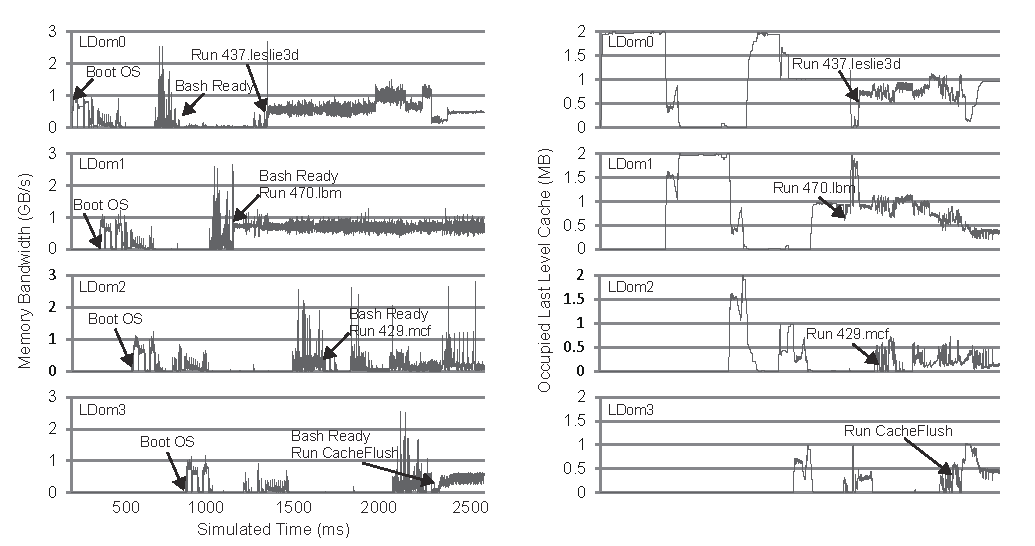
\includegraphics[width=\textwidth]{label/pard-nohype-simulator}
  \caption{动态划分一个PARD服务器为四个逻辑域,并在其中运行操作系统与应用}
  \label{fig:pard-nohype-simulator}
\end{figure}


\section{业界最新进展}
\label{chap:labeladdrspace:intel-rdt}

对于本章所分析的共享环境下多应用硬件资源竞争产生干扰的问题,
Intel从Xeon E5-v3系列处理器开始提供Resource Director Technology(RDT)\cite{intel-rdt}
方案来解决该问题。
如图\ref{fig:intel-rdt-overview}所示,该方案的硬件基础是资源监控与资源分配控制机制,
同时提供基于``监控$\rightarrow$策略$\rightarrow$控制''
组合的闭环方式来实现应用感知的资源管理框架。
其中资源监控提高了资源使用情况的能见度,使得资源利用率可以被跟踪,
同时可以侦测到应用性能随资源的变化,为上层的资源调度提供数据基础;
而硬件支持的资源分配控制机制,使得上层软件可以控制对硬件共享资源的使用。

% Intel RDT Overview
\begin{figure}[H]
  \centering
  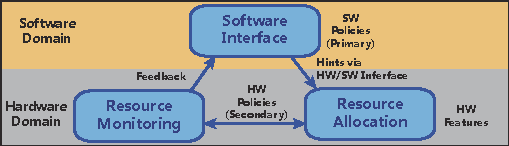
\includegraphics{x86eval/intel-rdt-overview}
  \caption[Intel Resource Director Technology (RDT) 技术示意图]{
    Intel Resource Director Technology (RDT)技术:硬件提供资源监控与分配功能,
    软件负责对资源使用进行调度,实现资源按需求动态分配。}
  \label{fig:intel-rdt-overview}
\end{figure}

目前Intel已经将RDT方案应用到共享末级缓存和内存控制器中,
在E5-v2系列中提供CMT和MBM功能(2013年),实现按应用区分的缓存容量监控,以及内存带宽监控;
在E5-v3系列中增加了CAT功能(2015年),实现按应用区分的缓存容量划分;
在E5-v4系列中扩展MBM功能(2016年),实现按应用区分的内存带宽监控。

CMT和MBM技术实现应用区分的缓存容量与内存带宽监控的流程如图\ref{fig:intel-cmt-flow}所示。
操作系统或VMM首先为执行实体(如线程、进程或虚拟机)分配资源编号RMID,后续的监控结果都将
以RMID的形式进行汇报。在OS/VMM执行调度并进行上下文切换时,将被调度实体的的RMID写入到目标
处理器核对应的寄存器中。OS/VMM可以随时通过RMID查询各个执行实体的资源使用情况,如共享缓存
占用或访存带宽等信息。
 
% Intel CMT Flow
\begin{figure}[H]
  \centering
  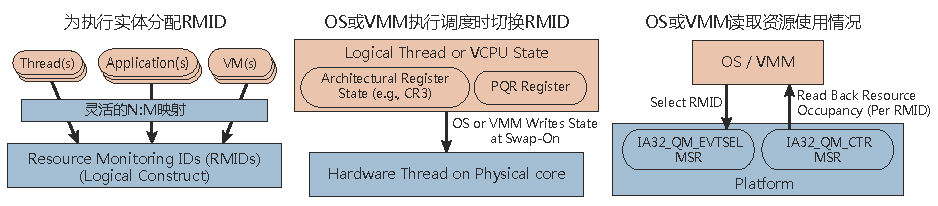
\includegraphics{x86eval/intel-cmt-flow}
  \caption[Intel Cache Monitor Technology (CMT) 技术流程]{Intel CMT技术流程:
   (1)为线程、应用或虚拟机等执行实体分配资源编号RMID;(2)将包含RMID的PQR寄存器
   保存在线程TCB或虚拟机VCPU中,并在执行上下文切换时写入到处理器核对应的物理寄存器中;
   (3)根据RMID使用MSRs寄存器获取共享资源使用情况。}
%Threads, applications, VMs or any combination can be associated with an RMID, enabling very flexible monitoring. As an example, all threads in a VM could be given the same RMID for simple per-VM monitoring. (2) The PQR register (containing an RMID) stored as part of a thread or VCPU state, which is written onto the thread-specific registers when a software thread is scheduled on a hardware thread for execution. (3) After a period of time (as defined by the software) the occupancy data for a given RMID can be read back through a pair of keyhole MSRs which provide the ability to input an RMID and Event ID (EvtID) in a selection MSR, and the hardware retrieves and returns the occupancy in the data MSR.}
  \label{fig:intel-cmt-flow}
\end{figure}

CAT技术为OS/VMM提供了控制末级共享缓存容量的功能,如图\ref{fig:intel-cat-flow}所示,
当该功能被开启后,应用将只能使用分配给它的Cache容量,实现路划分。
路划分策略是以COS为粒度进行指定,OS/VMM首先为某一COS制定路划分策略,并将该COS关联到使用
该策略的执行实体中,并在上下文划分时将被调度实体的COS写入到处理器核对应的寄存器中,
共享缓存根据COS对应的策略来进行缓存替换操作。

\begin{figure}[H]
  \centering
  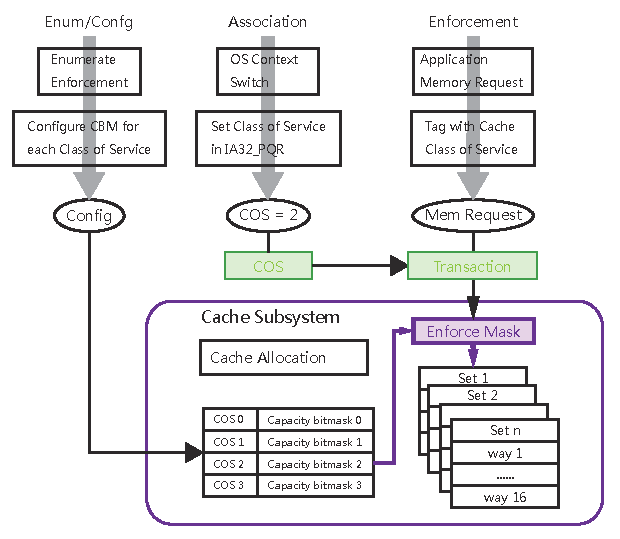
\includegraphics[height=8cm]{x86eval/intel-cat-flow}
  \caption[Intel Cache Allocation Technology (CAT) 技术流程]{Intel CAT技术流程}
  \label{fig:intel-cat-flow}
\end{figure}


\section{小结}

本章根据区分化服务的需求,分析了现有计算机体系结构的不足,提出使用标签传递软硬件信息,
让硬件支持区分化服务。并给出了标签化地址空间方案,包括标签的生成与传播,
同时使用模拟器验证了标签机制的可行性,并利用标签机制实现了全硬件支持的虚拟化。
最后,介绍业界在应用区分化服务方向上的最新进展,
Intel在其Xeon E5-v3(2015年)/v4(2016年)系列处理器提出的RDT技术,
使用与本章所述标签化地址空间相似的方案,
实现处理器末级缓存与内存控制器的性能监控、以及缓存容量划分。
未来数据中心计算机体系结构,标签将与地址具有相同的地位,
会成为体系结构内基本的元素。



